\documentclass[a4paper]{article}
\usepackage[pdftex]{graphicx}
\usepackage{anysize}
\marginsize{3cm}{3cm}{3cm}{3cm}
\linespread{1.2}
\usepackage[utf8]{inputenc}
\usepackage[T1]{fontenc}       
\usepackage[swedish]{babel}      
\usepackage{epstopdf}     % För svensk avstavning och svenska
\usepackage[osf]{mathpazo} % Palatino with smallcaps and oldstyle numbers
\usepackage[scaled]{helvet}

\usepackage{etoolbox}

\newcommand\getcurrentref[1]{%
 \ifnumequal{\value{#1}}{0}
  {??}
  {\the\value{#1}}%
}  
\newcommand\requirement[2]{
	\numberedrow{Krav}{#1}{#2}
}
\newcommand\scenario[2] {
	\numberedrow{Scenario}{#1}{#2}
}
\newcommand\numberedrow[3]{
	\noindent
	\textbf{#1 \getcurrentref{section}.\getcurrentref{subsection}.#2.} #3
	
}

\usepackage{fancyhdr}
\fancyhf{}
\fancyhead[L]{Ansvarig: SG}
\fancyhead[C]{Datum: \today}
\fancyhead[R]{Version: 0.11}


\title{SRS - Software Requirements Specification: NewPussSystem}                  	
\author{Systemarkitektgruppen \\ Lars Gustafsson | Martin Lichota | Marcel Tovar Rascon}
\date{}

\begin{document}

\maketitle
\thispagestyle{fancy}
\tableofcontents
\newpage

\section*{Dokumenthistorik}

\begin{tabular}{ l l l l }
Ver. & Datum & Ansv. & Beskrivning \\\hline
0.1 & 8 november 2014 & SG & Struktur för dokumentet\\
0.2 & 10 november 2014 & SG & Lägga till krav från UG\\
0.3 & 11 november 2014 & SG & Revidera krav samt ändra struktur\\
0.4 & 12 november 2014 & SG & Lade till nya samt reviderade krav\\
0.5 & 12 november 2014 & SG & Lade till nya samt reviderade krav\\
0.6 & 12 november 2014 & SG & Lade till nya samt reviderade krav\\
0.7 & 12 november 2014 & SG & Lade till nya samt reviderade krav\\
0.8 & 12 november 2014 & SG & Lade till nya samt reviderade krav\\
0.9 & 12 november 2014 & SG & Reviderade krav samt lade till scenarion\\
0.10 & 13 november 2014 & SG & Skapade scenarion för projektledning.\\
0.11 & 13 november 2014 & SG & Skapade scenarion för tidrapportmall och lade till krav.\\
\end{tabular}
\section{Inledning}       


Dokumentet beskriver kraven för <Program X>, ett tidsrapportingssystem för projekt som diverse användare kan logga in på.

\section{Referensdokument}
I denna version används inget referensmaterial.
\section{Bakgrund och mål}   
\subsection{Huvudmål}
Huvudmålet är att tillhandhålla ett system där olika användare, såsom projektledare och övriga projektmedlemmar, ska kunna tidsrapportera och loggföra det fortgående arbetet i sitt projekt. 

\subsection{Aktörer och deras mål}
Följande aktörer kommer att använda systemet:
\begin{itemize}
\item [] \textbf{Vanlig användare (User)} En användare kan logga in i systemet och tidsrapportera. Denne har även tillgång till statistik rörande den egna tidsrapporteringen.
\item [] \textbf{Administratör (Admin)} En administratör är en specifik användare som har privligerade rättigheter. Denne kan lägga till och ta bort andra användare.
\item [] \textbf{Projektledare (PL)} Projektledare är en roll som kan tilldelas till en User vilket ger den administrativa rättigheter för ett givet projekt.
\end{itemize}

\section{Terminologi}
Här följer ord och uttryck som används i rapporten och är till för att öka förståelsen.
\begin{itemize}
\item [Användarnamn] Unik indentifikationsfras för att representera en användare i systemet..
\item [Lösenord] Hemlig fras endast känd för var unik användare samt systemet så användaren kan påvisa sin identitet.
\item [Inloggad] En användare som har identifierat sig mot systemet med användarnamn och lösenord, detta sker genom att användaren loggar in.
\item [Logga in] Se inloggad.
\item [Användarstatus] En indikation på var användare som avgör hur vida den får logga in eller ej.
\item [Projektgrupp] En grupp bestående av vanliga användare och projektledare.
\item [Tidsrapport] En rapport som innehåller arbetsbelasting för en användare under en fix tidsperiod bundet till en specefik projektgrupp.
\item [Huvudsida] Med huvudsida avses den första vyn som användaren blir dirigerad till direkt efter inloggning. 
\item [Användarlista] En lista med alla användarnamn och lösenord som är sparade i databasen.
\end{itemize}
\section{Kontextdiagram}
Denna version innehålller inte ett kontextdiagram.
\section{Funktionella krav}
\subsection{Generella krav}
\label{krav-funk-gen}

 \requirement{1}{Systemet ska inte avbrytas eller låsa sig på grund av att användaren matar in en viss sekvens av data.}
\requirement{2}{Maximalt 50 användare kan vara inloggade på systemet samtidigt.}
\requirement{3}{Samtliga användare ska ha tillgång till följande funktionaliteter: start, tidrapportering, projektinformation, byta lösenord, hjälp samt utloggning.}
\requirement{4}{Systemarkitikter och projektledare ska utöver kraven i \ref{krav-funk-gen}.3 även ha tillgång till följande funktionaliteter: problemrapportering och statusrapportering.}
\requirement{5}{Samtliga funktionaliter i krav \ref{krav-funk-gen}.3 och \ref{krav-funk-gen}.4 ska vara tillgängliga i menyn enligt specifkiationerna som respektive krav anger.}
\requirement{6}{Menyn ska vara tillgänglig på samtliga sidor som visas av systemet.}
 
\subsection{Autentisering}
\label{krav-funk-aut}
\requirement{1}{För varje användare kan loginstatus antingen vara inloggad eller inte inloggad.}
\requirement{2}{Systemet ska hålla loginstatus i en serversession.}

% ----------------------- SCENARIO

\begin{table}[htbp]
\begin{tabular}{ | p{2cm} p{11cm} | }
   
        \hline
	\multicolumn{2}{|p{13cm}|}{ \indent\scenario{1}} \\
    \textbf{Syfte} & Logga in användaren i systemet.\\
    \textbf{Trigger} & Användaren inkommer till systemet. \\
    \textbf{Förutsättning} & Användaren är inte inloggad.\\
    \textbf{Frequency} & \\
    \textbf{Critical} & \\
    \hline

	\multicolumn{2}{|p{13cm}|}{ \textbf{Subuppgifter}:} \\

	\multicolumn{2}{|p{13cm}|}{ 1. Användaren får datafält för användarnamn och lösenord.}\\
	\multicolumn{2}{|p{13cm}|}{ 2. Användaren matar in användarnamn och lösernord och skickar data till servern genom ``Logga in''-knappen.} \\	
	\multicolumn{2}{|p{13cm}|}{ 3. Användarens loginstatus ändras till inloggad och är dirigerad till huvudsidan. }\\ \hline
    \multicolumn{2}{|p{13cm}|}{ \textbf{Varianter}: }\\
	\multicolumn{2}{|p{13cm}|}{ 3.a Det givna användarnamnet och lösernordet matchar inte något par i systemets databas. Detta meddelas då till användaren som får repetera inloggningen.}\\
	    \hline


\end{tabular}
\end{table}
% ----------------------- /END

\requirement{3}{När en användare når systemet och inte är inloggad ska denne få en förfrågan om användarnamn och lösenord.}
\requirement{4}{När en användare skickar ett användarnamn och lösenord ska dessa parametrar jämföras med användarlistan och om användaren ska få tillgång till systemet , så ska serverstatus ändras till ``inloggad'' och huvudsidan ska visas.}
\requirement{5}{Ingen information som kräver inloggning får visas för en oninloggad användare.}


% ----------------------- SCENARIO
\begin{table}[htbp]
\begin{tabular}{ | p{2cm} p{11cm} | }
   
        \hline

    \multicolumn{2}{|p{13cm}|}{ \indent\scenario{2}} \\
    \textbf{Syfte} & Logga ut användaren från servern.\\
    \textbf{Trigger} & Användaren trycker väljer att logga ut. \\
    \textbf{Förutsättning} & Användaren är inloggad.\\
    \textbf{Frequency} & \\
    \textbf{Critical} & \\
    \hline
	\multicolumn{2}{|p{13cm}|}{ \textbf{Subuppgifter}:} \\
	\multicolumn{2}{|p{13cm}|}{ 1. Användaren väljer logga ut länken i menyn och loggas ut, samt dirigeras till en sida där utloggningen bekräftas.}\\ \hline
    \multicolumn{2}{|p{13cm}|}{\textbf{Varianter}: }\\
	\multicolumn{2}{|p{13cm}|}{1.a Användaren har redan blivit utloggad från servern. I sådana fall meddelas detta till användaren som dirigeras till utloggningssidan.} \\
	    \hline


\end{tabular}
\end{table}
% ----------------------- /END


\requirement{6}{Om en inloggad användare är inaktiv i längre än 20 minuter ska sagda användare loggas ut och tvingas att logga in igen innan fortsatt användning av systemet.}
\requirement{7}{Ett användarkonto kan endast vara inloggat på en enhet åt gången.}
\requirement{8}{Om en användare försöker logga in med ett användarkonto som redan är inloggat på en annan enhet, kommer den nya inloggingen att genomföras medan den andra enheten loggas ut.}
\requirement{9}{Scenario \ref{krav-funk-aut}.1 skall stödjas av systemet.}
\requirement{10}{Scenario \ref{krav-funk-aut}.2 skall stödjas av systemet.}
\subsection{Data}
\label{krav-funk-data}
\requirement{1}{Användarnamn ska bestå av 5-10 tecken, ascii (decimal) värden 48-57, 65-90, och 97-122 är tillåtna.}
\requirement{2}{Användarnamn måste vara unika.}
\requirement{3}{Lösenord ska bestå av sex tecken, ascii (decimal) värden 97-122 är tillåtna.}
\requirement{4}{Tidrapportering sker i antal minuter.}
\requirement{5}{Tidrapportens utseende, med avseende på vilka aktiviteter man kan föra in tidinformation i, bestäms av administratören innan projektgruppen har skapats. När projektet är skapat ska det inte gå att ändra tidrapportens utseende.}
\requirement{6}{Tidrapportens grundmall ska innehålla information om användarnamn, projektnamn, datum och veckonummer. Det ska även tydligt framgå om den är signerad eller ej. Grundmallen genereras automatiskt av systemet.}
\requirement{7}{Samtliga tidrapportmallar sparas på servern.}
\requirement{8}{Maximalt 20 mallar kan lagras samtidigt, därefter skrivs de över enligt FIFO-principen.}
\requirement{9}{En tidrapportmall ska bestå av 1-10 rader samt 1-5 kolumner som det går att mata in tidinformation i.}
\requirement{10}{Namnet på tidrapportmallen ska bestå av 5 tecken, ascii (decimal) värden 48-57 och 97-122 är tillåtna.}
\requirement{11}{Namnet på aktivitet och subaktivitet ska bestå av 3-5 tecken respektive 1 tecken, ascii (decimal) värden 48-57 och 97-122 är tillåtna.}



\subsection{Administration}
\label{krav-funk-admin}

\begin{figure}[h!]
  \centering
    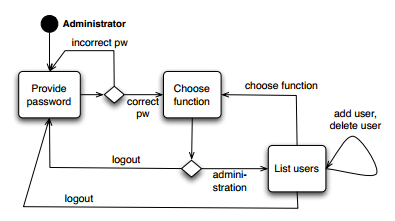
\includegraphics[width=0.5\textwidth]{admin_usage}
   \caption{A picture of a gull.}
   \label{image_admin_usage}
\end{figure}
\requirement{1}{Systemet ska stödja sekvensen för administrören som visas i Figur \ref{image_admin_usage}.}
\requirement{2}{Det skall finnas en och endast en administratör med användarnamnet ''admin'' och lösenordet ''adminpw''.}
\requirement{3}{Som inloggad administratör skall det vara möjligt att välja administrationsvyn på huvudsidan.}
\requirement{4}{En ny användare, skapad av administratören, måste ha ett unikt användarnamn samt bli tilldelad ett slumpmässigt lösenord från systemet.}
\requirement{5}{Om administratören försöker att lägga till en användare med ett användarnamn som redan existerar i systemet, skall användaren inte läggas till och ett felmeddelande skall visas.}
\requirement{6}{Om en administratör väljer administrationsvyn skall denne få åtkomst till administationsverktygen, men om samma val görs av en ickeadministratör skall denne istället få åtkomst till huvudsidan.}
\requirement{7}{I administrationsvyn skall alla användare listas med både användarnamn och lösenord.}
\requirement{8}{I administrationsvyn skall det vara möjligt att ta bort vilken användare som helst förutom administratören.}
\requirement{9}{Varje borttagning av en användare skall bekräftas av en dialogruta frågandes om man är säker. Om administratören väljer ``Ja'', tas användaren bort och administratören kommer tillbaka till en uppdaterad lista med användarna. Om ``Nej'' väljs, går administratören tillbaka till nuvarande sida.}
\requirement{10}{I administrationsvyn skall det vara möjligt att lägga till en ny användare.}
\requirement{11}{Om en administratör försöker lägga till en ny användare med ett användarnamn som strider mot krav \ref{krav-funk-data}.1-2 skall ett felmeddelande visas och användaren skall inte läggas till.}
\requirement{12}{Endast administratören skall kunna skapa projektgrupper i systemet.}
\requirement{13}{Då en ny projektgrupp skapas skall administratören ange ett gruppnamn, projektledare och eventuella gruppmedlemmar.}
\requirement{14}{Om administratören försöker skapa en projektgrupp med ett namn som redan existerar skall projektgruppen inte skapas och ett felmeddelande skall visas.}
\requirement{15}{Endast administratören skall kunna ta bort projektgrupper i systemet.}
\requirement{16}{När en projektgrupp tas bort skall administratör kunna välja projektgrupp ur en lista på alla projektgrupper i systemet.}
\requirement{17}{Administratören ska kunna ändra gruppmedlemmar i en existerande projektgrupp.}
\requirement{18}{Administratören ska kunna ändra gruppmedlemmars roller i en existerande projektgrupp.}
\requirement{19}{Administratören ska kunna utforma en tidrapportmall. Se även krav \ref{krav-funk-data}.5 och \ref{krav-funk-data}.6.}


%--------------SCENARIO

\begin{table}[htbp]
\begin{tabular}{ | p{2cm} p{11cm} | }
    \hline
    
    \multicolumn{2}{|p{13cm}|}{ \indent\scenario{1}} \\
    \textbf{Syfte} & Skapa tidrapportmall.\\
    \textbf{Trigger} & Användaren vill skapa en projektgrupp. \\
    \textbf{Förutsättning} & Användaren måste vara inloggad som administratör.\\
    \textbf{Frequency} & \\
    \textbf{Critical} & \\
    \hline

	\multicolumn{2}{|p{13cm}|}{\textbf{Subuppgifter}:} \\

	\multicolumn{2}{|p{13cm}|}{1. Användaren väljer att skapa projektgrupp.}\\
	\multicolumn{2}{|p{13cm}|}{2. Användaren väljer att skapa en ny tidrapportmall.} \\	
	\multicolumn{2}{|p{13cm}|}{3. Denne väljer antal aktiviteter (rader) och subaktiviteter (kolumner) som ska finnas. Användaren fyller i önskat namn på tidrapportmallen och trycker ''OK''.} \\	
	\multicolumn{2}{|p{13cm}|}{4. Tabell genereras med det antal givna rader och kolumner från steg 3 och visas för användaren.} \\	
	\multicolumn{2}{|p{13cm}|}{5. Användaren fyller nu i aktivitets- och subaktivitetsnamn. Därefter trycker denne ''OK''.} \\	
	\multicolumn{2}{|p{13cm}|}{6. Mallen är nu skapad och sparad. Användaren får en bekräftelse och dirigeras till den färdiga mallen.} \\	
	\hline
    \multicolumn{2}{|p{13cm}|}{\textbf{Varianter}: }\\
    \multicolumn{2}{|p{13cm}|}{2a. Användaren väljer att använda en befintlig tidrapportmall.}\\
    \multicolumn{2}{|p{13cm}|}{3a. Om namnet på mallen redan existerar informeras användaren och ombedes att skriva ett annat namn.}\\
    \multicolumn{2}{|p{13cm}|}{4a. Användaren får felmeddelande då antal kolumner och rader överstiger specifieringen i krav \ref{krav-funk-data}.9. Användaren skickas tillbaka till steg 3.}\\
       \multicolumn{2}{|p{13cm}|}{4b. Användaren får felmeddelande då det inmatade namnet strider mot krav \ref{krav-funk-data}.10. Användaren skickas tillbaka till steg 3.}\\
    \multicolumn{2}{|p{13cm}|}{6a. Användaren får felmeddelande då det inmatade aktivitets- eller subaktivitetsnamnet strider mot krav \ref{krav-funk-data}.11. Användaren skickas tillbaka till steg 5.}\\
    \hline
\end{tabular}
\end{table}

% ----------------------- /END


\subsection{Tidrapportering}
\label{krav-funk-tid}

\requirement{1}{Nygenererade tidrapporter är alltid osignerade.}
\requirement{2}{Användaren skall kunna skapa, uppdatera och ta bort sina egna osignerade tidrapporter för de projekt den är medlem i.}
\requirement{3}{Användaren kan inte ta bort eller redigera sina signerade rapporter.} 
\requirement{4}{En användare som inte är projektledare kan bara se sina egna rapporter.}

\requirement{5}{Användaren ska kunna föra in information enligt krav \ref{krav-funk-data}.4. }
\requirement{7}{Scenario \ref{krav-funk-tid}.1 skall stödjas av systemet.}

%--------------SCENARIO

\begin{table}[htbp]
\begin{tabular}{ | p{2cm} p{11cm} | }
    \hline
    
    \multicolumn{2}{|p{13cm}|}{ \indent\scenario{1}} \\
    \textbf{Syfte} & Dokumentera arbetstimmar i systemet.\\
    \textbf{Trigger} & Användaren kommer in på tidrapporteringssidan. \\
    \textbf{Förutsättning} & Användaren måste vara medlem i ett projekt.\\
    \textbf{Frequency} & \\
    \textbf{Critical} & \\
    \hline

	\multicolumn{2}{|p{13cm}|}{\textbf{Subuppgifter}:} \\

	\multicolumn{2}{|p{13cm}|}{1. Användaren väljer tidrapportering i menyn.}\\
	\multicolumn{2}{|p{13cm}|}{2. Ett fält var användaren kan fylla i veckonummer för veckan som skall rapporteras 	visas. Under fältet framgår det för vilken vecka senaste rapporten var skapad/reviderad.} \\	
	\multicolumn{2}{|p{13cm}|}{3. Användaren fyller i veckonummer och trycker OK.} \\
	\multicolumn{2}{|p{13cm}|}{4. En ny tidrapport genereras och visas med veckonumret från föregående steg i fyllt.} \\
	\multicolumn{2}{|p{13cm}|}{5. Användaren kan nu fylla i tidinformation. }\\

	\multicolumn{2}{|p{13cm}|}{6. Användaren bekräftar slutligen genom att trycka på ”Skicka”, längst ner på sidan.}\\
	
	\multicolumn{2}{|p{13cm}|}{8. Rapporten sparas i databasen. En bekräftelse på att så har skett visas för användaren. Användaren kan även notera totaltiden.}\\ \hline
    \multicolumn{2}{|p{13cm}|}{\textbf{Varianter}: }\\
	\multicolumn{2}{|p{13cm}|}{2a. Det finns ingen tidigare skapad rapport. Detta framgår under fältet. }\\
	\multicolumn{2}{|p{13cm}|}{4a. En tidrapport för det ifyllda veckonumret existerar redan. Rapporten hämtas från 		databasen och visas för användaren. Denne kan nu redigera rapporten. }\\
	\multicolumn{2}{|p{13cm}|}{8a. Rapporten sparades inte i databasen. Användaren får information om detta och skickas tillbaka, utan att någon information i fälten har gått förlorad.}\\
    \hline
\end{tabular}
\end{table}

% ----------------------- /END



\subsection{Projektledning}
\label{krav-funk-proj}
\requirement{1}{Varje projekt skall ha två, och endast två användare, som besitter rollen som projektledare.}
\requirement{2}{Projektledaren skall ha tillgång till samtliga projektmedlemmars tidrapporter i sin projektgrupp.}
\requirement{3}{Projektledaren skall kunna godkänna ej tidigare godkända tidrapporter i från medlemmar i sin projektgrupp.}
\requirement{4}{Projektledaren skall kunna ta tillbaka sitt godkännande från en tidigare godkänd gruppmedlems tidsrapport, i sin projektgrupp.}
\requirement{5}{Projektledaren skall kunna generera statistik över sitt projekt genom att göra något av följande; summera alla tidrapporter, summera tidrapporter per användare/roll/aktivitet/vecka.}

%--------------SCENARIO

\begin{table}[htbp]
\begin{tabular}{ | p{2cm} p{11cm} | }
    \hline
    
    \multicolumn{2}{|p{13cm}|}{ \indent\scenario{1}} \\
    \textbf{Syfte} & Generera rapporter från systemet.\\
    \textbf{Trigger} & En användare kommer in på statistiksidan för sitt projekt. \\
    \textbf{Förutsättning} & Användaren måste vara projektledare för det givna projektet.\\
    \textbf{Frequency} & \\
    \textbf{Critical} & \\
    \hline

	\multicolumn{2}{|p{13cm}|}{\textbf{Subuppgifter}:} \\

	\multicolumn{2}{|p{13cm}|}{1. Användaren väljer statistik i menyn.}\\
	\multicolumn{2}{|p{13cm}|}{2. Användaren väljer från en lista vilken typ av rapport den vill generera.} \\	
	\multicolumn{2}{|p{13cm}|}{3. En rapport genereras med statistik efter användarens önskemål} \\	
	\hline
    \multicolumn{2}{|p{13cm}|}{\textbf{Varianter}: }\\
    \hline
\end{tabular}
\end{table}

% ----------------------- /END

\requirement{6}{Projektledaren skall kunna tilldela egenbestämda roller till gruppmedlemmarna i sin projektgrupp.}
\requirement{7}{Scenario \ref{krav-funk-proj}.1 skall stödjas av systemet.}

\section{Kvalitetskrav}
\subsection{Underhåll}
\requirement{1}{Systemet skall vara väl dokumenterad så det underlättar vidareutvekling av systemet i framtiden.}
\requirement{2}{Förståelse av Java, i nivå med vad som lärs ut i kursen EDA016, samt grundläggande kunskap av SQL skall räcka för att underhålla samt vidareutvekla systemet.}
\subsection{Prestanda}
\requirement{1}{Då systemet används i en av datorsalarna I ``E-huset'', LTH, skall svaret på en godtycklig förfrågan i åtminstone 95\% av fallen ges inom 1,0 s.}
\section{Projektkrav}
\subsection{Utvecklingsmiljö}
\requirement{1}{Systemet skall vara utveklat för Apaches Tomcat server.}
\requirement{2}{Systemet skall vara utveklat i Java.}
\requirement{3}{Databaslösningen MySQL skall användas av programmet för lagring av data mellan sessioner.}
\requirement{4}{Systemet samt projekt- och produktdokumentation skall skrivas på svenska. Java-koden skall följa standarden som finns på http://www.geosoft.no/development/javastyle.html, alla variabelnamn skall vara skrivna på engelska.}

\end{document}